\section{A fixed seven-step forcing}
\label{sec:seven-step}

Fix the impulse and height words
\[
 d=(0,0,1,-1,0,1,-1),\qquad
 h=(0,0,0,1,0,0,1),
\]
with $d_i=h_{i+1}-h_i$ and phase indices read modulo seven.
Write $F=F_d$ for the physical update in \eqref{eq:physical-forcing}, including at zero.
The safe domain

\[
 \mathcal D=\{(n,i):n\ge h_i\}
\]
contains every positive initial integer at every phase, together with
zero at the five phases where $h_i=0$.

By Proposition~\ref{prop:height-conjugacy}, $z=n+1-h_i$ evolves on
the positive integers under the repeated word $UUUTUUT$.

The phase-indexed physical values
\begin{equation}
 (c_0,c_1,c_2,c_3,c_4,c_5,c_6)=(0,0,0,1,1,2,2)
 \label{eq:seven-cycle}
\end{equation}
form a cycle: $T(c_i)+d_i=c_{i+1}$ at every phase.  In positive
coordinates its successive states are
\[
 (1,0),(1,1),(1,2),(1,3),(2,4),(3,5),(2,6).
\]
We say that a state is \emph{captured} if its forward orbit visits one
of the states $(c_i,i)$, and write $\operatorname{Cap}(n,i)$ for this
property.

\subsection{Section states and the exact open obligations}

Consider the section
\[
 \mathcal S=\{(z,i):z=3m,\ m\ge1,\ i\in\{3,5,6\}\}.
\]
For clarity, a pair $(m,i)$ in a section formula denotes the physical
state
\begin{equation}
 s(m,i)=(3m-1+h_i,i).
 \label{eq:seven-section-launch}
\end{equation}
Let $P$ denote the first \emph{strictly later} visit to $\mathcal S$.
A visit after a shrinking step counts.  Return existence will be proved
below, independently of capture.

The relevant natural-valued ranks are
\begin{align}
 V(m,3)&=V(m,5)=m,& V(m,6)&=2m,\\
 \rho(m,i)&=2V(m,i)+\mathbf1_{\{i=6\}}.
 \label{eq:seven-rho}
\end{align}
The same rank is used for all section phases simultaneously.

\begin{theorem}[Four-family conditional capture]
\label{thm:seven-four}
For the fixed forcing $d$, the following are equivalent.
\begin{enumerate}
\item Every positive physical integer, at every initial phase, is captured
by \eqref{eq:seven-cycle}.
\item Each of the following four statements holds:
\begin{align*}
 \mathrm{S00}:&\quad
 \operatorname{Cap}(s(4t+3,3))\quad &&\text{for every }t\ge0,\\
 \mathrm{S01}:&\quad
 \operatorname{Cap}(s(2t,5)) &&\text{for every }t\ge1,\\
 \mathrm{S02}:&\quad
 \operatorname{Cap}(s(32t+3,5)) &&\text{for every }t\ge0,\\
 \mathrm{S03}:&\quad
 \operatorname{Cap}(s(128t+115,5)) &&\text{for every }t\ge0.
\end{align*}
\end{enumerate}
In the second display, $\operatorname{Cap}(s(m,i))$ means capture of the
physical state defined in \eqref{eq:seven-section-launch}.  Equivalently,
every failure of capture would give a least-$\rho$ failure in this
four-family union.  None of the four universal hypotheses is discharged
by the theorem.
\end{theorem}

\subsection{Affine certificates on residue classes}

Every computational check in the reduction uses an input of the form
\[
 z=Aq+B,\qquad q\ge q_0,
\]
and propagates the two coefficients exactly.  When $A$ is even, every
input in this domain has the parity of $B$.  A physical shortcut step
therefore acts on the entire domain by
\[
 (a,b)\longmapsto
 \begin{cases}
 (a/2,b/2+d_i),&b\text{ even},\\
 (3a/2,(3b+1)/2+d_i),&b\text{ odd}.
 \end{cases}
\]
Here $(a,b)$ are physical-coordinate coefficients; the checker first
substitutes $n=z-1+h_i$ and converts back after each step.  At a candidate
section phase, the free coefficient remains divisible by three.  Hence
membership in the section is decided for the entire domain by the
constant coefficient modulo three.  Safety is checked at $q_0$ together
with positivity of the coefficient.

For the entrance calculation we use $A=384=3\cdot2^7$ and at most
seven updates.  For the short-return calculation from phase $i$ we use
$A=3\cdot2^{L_i}$ and at most $L_i$ updates.  The factor $2^{L_i}$
fixes every required parity; multiplying by an odd integer at a step
does not consume any additional powers of two.  The factor of three
fixes all section tests.  Each computation therefore covers the full ray.

An affine inequality on $q\ge q_0$ follows by checking that its slope
is nonnegative and its value at $q_0$ is nonnegative; strict inequalities
are treated with the corresponding integer minimum.  A negative slope
cannot be discarded by testing only small $q$.  The complete residue
partitions below use $0\le B<A$, with $q_0=1$ when the initial positive
coordinate would otherwise be zero.

\subsection{Every orbit reaches the section}

Start at phase zero, with $z=384q+r$, $0\le r<384$.  Propagate the
physical recurrence until a section hit or the end of one period.
Exactly 370 residue domains hit the section.  The fourteen remaining
domains have the following full-period returns; the output is $aq+b$.
All entries in this table have $q\ge0$.
\begin{center}
\begin{tabular}{rrr|rrr}
\hline
$r$&$a$&$b$&$r$&$a$&$b$\\ \hline
3&27&2&195&9&5\\
9&9&2&201&3&2\\
44&81&11&236&27&17\\
67&9&2&259&27&20\\
108&27&8&300&81&65\\
131&27&11&323&9&8\\
172&81&38&364&27&26\\ \hline
\end{tabular}
\end{center}
In each row $a<384$ and $1\le b<r$.  An avoiding period therefore
strictly lowers the positive integer $z$.  Indefinite avoidance would
produce an infinite strictly decreasing sequence of positive integers,
which is impossible.  An arbitrary initial phase can be aligned to zero
in at most six updates if no earlier section hit occurs.  This proves
entry from every state in $\mathcal D$.  Applying entry after one
further physical update proves that $P$ is total on $\mathcal S$.

The fourteen returns also satisfy the common envelope
\begin{equation}
 z_{\mathrm{next}}\le f(z):=\frac{27z+220}{128},
 \qquad f\left(\frac{220}{101}\right)=\frac{220}{101}.
 \label{eq:seven-avoid-envelope}
\end{equation}
This follows row by row by comparing coefficients and constants.
The 370 exiting domains satisfy
\begin{equation}
 w_j z_{\mathrm{exit}}\le\frac{27}{8}z,
 \qquad (w_3,w_5,w_6)=(1,1,2),
 \label{eq:seven-exit-envelope}
\end{equation}
where $j$ is the phase of the first section hit.  The factor at phase six is two.

\subsection{All sufficiently long returns strictly descend}

From a phase-five section launch, either the section is hit during
alignment or the phase-zero value is at most $(3z+5)/4$.  From phase
six, its phase-zero value is at most $(3z+1)/2$.  These two bounds use
respectively two and one updates and follow from the four and two
fixed-parity domains.

If there is then one complete avoiding period before the next section
hit, composing these bounds with \eqref{eq:seven-avoid-envelope} and
\eqref{eq:seven-exit-envelope} gives
\begin{align}
 w_jz_{\mathrm{exit}}
 &\le\frac{2187z+27405}{4096}<z
 &&\text{from phase five, if }z\ge15,\\
 w_jz_{\mathrm{exit}}
 &\le\frac{2187z+12609}{2048}<2z
 &&\text{from phase six, if }z\ge9.
 \label{eq:seven-long-bounds}
\end{align}
For example, the first strict inequality is equivalent to
$1909z>27405$ and holds already at $z=15$.  Its left-hand side
increases thereafter.  The second is equivalent to $1909z>12609$
and holds at $z=9$.

These estimates cover arbitrarily many avoiding periods.  Indeed,
the initial alignment upper bound is above $220/101$ at the stated
threshold.  Since $f$ is increasing and contracts towards that fixed
point, $f^k(B)\le f(B)$ for every $k\ge1$ and every such initial
bound $B$.  Applying the weighted exit estimate after the last avoiding
period therefore gives the same upper bound for every possible wait.

The last update of a phase-zero period ends at phase zero, which is
outside $\mathcal S$.  Consequently a return later than alignment
plus six updates entails a full avoiding period.  At phase three all
returns occur within three updates; the following complete table on
$m=8q+r$ verifies this directly:
\begin{center}
\begin{tabular}{rrrr}
\hline
$r$&output parameter&output phase&updates\\ \hline
0&$6q$&5&2\\
1&$6q+1$&5&2\\
2&$3q+1$&6&3\\
3&$18q+7$&5&2\\
4&$6q+3$&5&2\\
5&$6q+4$&5&2\\
6&$q+1$&6&3\\
7&$18q+16$&5&2\\ \hline
\end{tabular}
\end{center}
Here $q\ge1$ in the first row and $q\ge0$ in the others.
Thus every first return failing to strictly decrease $V$, apart from
the explicitly handled small inputs, occurs within the caps
\begin{equation}
 L_3=3,\qquad L_5=8,\qquad L_6=7.
 \label{eq:seven-caps}
\end{equation}
The small inputs outside the thresholds in \eqref{eq:seven-long-bounds}
have the exact returns
\begin{center}
\begin{tabular}{rrr}
\hline
launch $(m,i)$&return $(m',j)$&updates\\ \hline
$(1,5)$&$(1,5)$&7\\
$(2,5)$&$(3,6)$&1\\
$(3,5)$&$(9,3)$&5\\
$(4,5)$&$(6,6)$&1\\
$(1,6)$&$(1,3)$&4\\
$(2,6)$&$(1,3)$&11\\ \hline
\end{tabular}
\end{center}
The eleven-update return from $(2,6)$ lowers $V$ from $4$ to $1$.

\subsection{A complete direct first-return classification}

Use the residue partitions $m=2^{L_i}q+r$ at phases $i=3,5,6$.
There are $8+256+128=392$ infinite input domains.  The exact propagation
described above stops at the first later section visit.  Domains that
have not returned by their cap are covered by the long-return proof.
All other outputs are affine in $q$, so their rank differences can
be classified on the entire legal ray.

The six direct growing families are as follows.  Parameters are
nonnegative except for S01, where $t\ge1$.
\begin{center}
\begin{tabular}{llllr}
\hline
ID&launch $(m,i)$&return $(m',j)$&$V_{\rm out}-V_{\rm in}$&updates\\ \hline
S00&$(4t+3,3)$&$(9t+7,5)$&$5t+4$&2\\
S01&$(2t,5)$&$(3t,6)$&$4t$&1\\
S02&$(32t+3,5)$&$(81t+9,3)$&$49t+6$&5\\
S03&$(128t+115,5)$&$(243t+220,5)$&$115t+105$&7\\
S06&$(16t+7,6)$&$(81t+36,3)$&$49t+22$&4\\
S08&$(64t+15,6)$&$(243t+58,5)$&$115t+28$&6\\ \hline
\end{tabular}
\end{center}
These labels match the certificate files. The six families occupy
respectively $2,128,8,2,8,2$ of the fixed-modulus input domains.
Nine domains require the long-return argument.  On every other domain
the first return strictly lowers $V$, except possibly at the three
individual launches
\begin{equation}
 (m,i)=(1,3),(2,3),(1,5).
 \label{eq:seven-finite-base}
\end{equation}
For a domain containing one of these launches, every larger parameter
strictly descends.

The exact chains
\[
 (1,3)\xrightarrow{2}(1,5),\qquad
 (2,3)\xrightarrow{3}(1,6)\xrightarrow{4}(1,3)
               \xrightarrow{2}(1,5)
\]
settle \eqref{eq:seven-finite-base}; the arrows count literal updates.
The launch $(1,5)$ lies on the cycle \eqref{eq:seven-cycle} and
returns to itself after seven updates.

For an illustration of a whole growing-parameter case that the rank
already resolves, the first return
\[
 (64t+63,6)\longmapsto(81t+80,5),\qquad t\ge0,
\]
has an unweighted parameter increase but a strict $V$-decrease
$47t+46$, so this launch cannot minimize the rank of an uncaptured state.

\subsection{A merger closes the two phase-six induction cases}

Suppose $m=4q+3$ and set $x=3m=12q+9$, so $x\equiv1\pmod4$.
The positive-coordinate launch $(x,6)$ follows its prescribed two
steps as
\[
 (x,6)\longmapsto\left(\frac{3x+1}{2},0\right)
       \longmapsto\left(\frac{9x+3}{4},1\right).
\]
The alternative section launch $(2x,5)$ follows three prescribed
steps as
\[
 (2x,5)\longmapsto(3x,6)
       \longmapsto\left(\frac{9x+1}{2},0\right)
       \longmapsto\left(\frac{9x+3}{4},1\right).
\]
The indicated parities follow from $x\equiv1\pmod4$.  Both histories
are positive and meet at the same integer and the same phase.  In
physical coordinates this common state is $(27q+20,1)$.  Their future
orbits therefore agree, although their elapsed times differ.

The old ranks of the launches tie, but the refined rank has
\begin{equation}
 \rho(m,6)-\rho(2m,5)=(4m+1)-4m=1.
 \label{eq:seven-merger-gap}
\end{equation}
Both S06 and S08 satisfy $m\equiv3\pmod4$ throughout their domains.
Their alternate section parameters are respectively $32t+14$ and
$128t+30$, at phase five.  Their common positive-coordinate states
are respectively $(108t+48,1)$ and $(432t+102,1)$.

Every old strict $V$-decrease survives this refinement.  Indeed,
$V(a)-V(b)\ge1$ implies
\[
 \rho(a)-\rho(b)
 =2\bigl(V(a)-V(b)\bigr)+\mathbf1_{\{i_a=6\}}
                         -\mathbf1_{\{i_b=6\}}\ge1.
\]
This argument covers all long returns as well as the short affine
domains.  It does not cover equal-$V$ transitions automatically.  In
particular, the finite step $(2,3)\to(1,6)$ increases $\rho$ from
$4$ to $5$; it is valid because its explicit finite capture chain
has already been proved, not because it decreases the rank.

The table counts fixed-modulus domains after the merger. The column labelled ``finite'' counts
domains with a single exceptional base input; the rest of such a
domain strictly descends.
\begin{center}
\begin{tabular}{rrrrrrr}
\hline
phase&domains&forward&long&merger&residual&finite\\ \hline
3&8&4&0&0&2&2\\
5&256&113&4&0&138&1\\
6&128&113&5&10&0&0\\ \hline
\end{tabular}
\end{center}
Thus no least-$\rho$ failure can occur at phase six.  This does not
remove S01 automatically: its phase-six return has greater rank
than the original S01 launch.  Any composed rule must be compared
against the original rank.

\begin{proof}[Proof of Theorem~\ref{thm:seven-four}]
Every launch in the four hypotheses is a positive physical state,
so universal positive-seed capture implies the four hypotheses.
For the converse, assume them.  If any state in $\mathcal D$ failed
capture, section entry would provide a failed section state.  Choose
one of least natural-valued rank $\rho$.  It is not one of
\eqref{eq:seven-finite-base}, since those states are captured.
It is not in S00--S03 by hypothesis.  Every other section state
either has a strict rank-decreasing forward return, or belongs to
S06 or S08 and has a phase-correct merger with the smaller-ranked
alternative launch above.  In either case the smaller state has
the same failed future.  This contradicts minimality.  Hence every
state in $\mathcal D$, and in particular every positive physical
seed at every phase, is captured.
\end{proof}

For each remaining launch $a$, it suffices to show capture or exhibit a
section launch $b$ with $\rho(b)<\rho(a)$ and $F^u(a)=F^v(b)$ for
some $u,v\ge0$. Equality includes the phase. Shaw's impure integers
have a smaller positive predecessor under the unshortened odd update
$3n+1$ \cite[Definition~2.1 and Theorem~3.1]{shaw-2006}. Here the two
orbits may meet later, at different update counts, and $\rho$ compares
their initial states.

\subsection{Optimality of direct phase-affine ranks}

\begin{proposition}[Six direct growing domains are unavoidable]
\label{prop:seven-six-barrier}
There is an explicit set of eleven pairwise disjoint first-return
affine domains of $P$ such that, for every choice of positive real
weights $w_3,w_5,w_6$ and fixed real constants $c_3,c_5,c_6$, the
rank $R(m,i)=w_i m+c_i$ strictly increases on an infinite tail of at
least six of those domains.  For $V$, exactly the six S-domains in
this witness set grow; the complete classifier above has no other
growing tails.
\end{proposition}

\begin{proof}
In addition to the six S-domains already listed, the following five
domains are first returns.  All parameters are nonnegative except
for D35, where $t\ge1$.
\begin{center}
\begin{tabular}{lllr}
\hline
ID&launch $(m,i)$&return $(m',j)$&updates\\ \hline
D53&$(32t+31,5)$&$(27t+27,3)$&5\\
D35&$(4t+1,3)$&$(3t+1,5)$&2\\
D36&$(8t+2,3)$&$(3t+1,6)$&3\\
D65&$(8192t+6239,6)$&$(6561t+4999,5)$&13\\
D56&$(256t+147,5)$&$(81t+47,6)$&8\\ \hline
\end{tabular}
\end{center}
These eleven domains are pairwise disjoint: at a common phase their
residues disagree modulo the greatest common divisor of their input
moduli.  The bundled checker verifies their exact parities, safety,
endpoints, and absence of earlier section visits on every parameter.

For a branch $(Mt+r,i)\to(At+b,j)$ the leading coefficient of
$R_{\mathrm{out}}-R_{\mathrm{in}}$ is $w_jA-w_iM$.
If every coefficient on a directed phase cycle were nonpositive,
multiplying the inequalities would force the product of the
unweighted slopes $A/M$ to be at most one.  The following six
edge-disjoint cycles violate that bound:
\begin{center}
\begin{tabular}{lr}
\hline
cycle&product of slopes\\ \hline
S03&$243/128$\\
S00, D53&$243/128$\\
S02, D35&$243/128$\\
S06, D36&$243/128$\\
S01, D65&$19683/16384$\\
S08, D56&$19683/16384$\\ \hline
\end{tabular}
\end{center}
Every product exceeds one.  Hence each cycle contains a domain
with a strictly positive leading rank change.  The fixed offsets
cannot remove growth on its infinite tail.  Disjointness gives six
different input domains.  For $V$, the six S-domain leading changes
are positive and the five D-domain leading changes are negative.
The complete direct classification already excludes other growing
tails.
\end{proof}

The cycles constrain the rank weights. Their guards need not form
periodic trajectories. The count concerns the specified disjoint
domains on this section and leaves residue-dependent ranks, later
returns, and mergers available.

\begin{figure}[tbp]
\centering
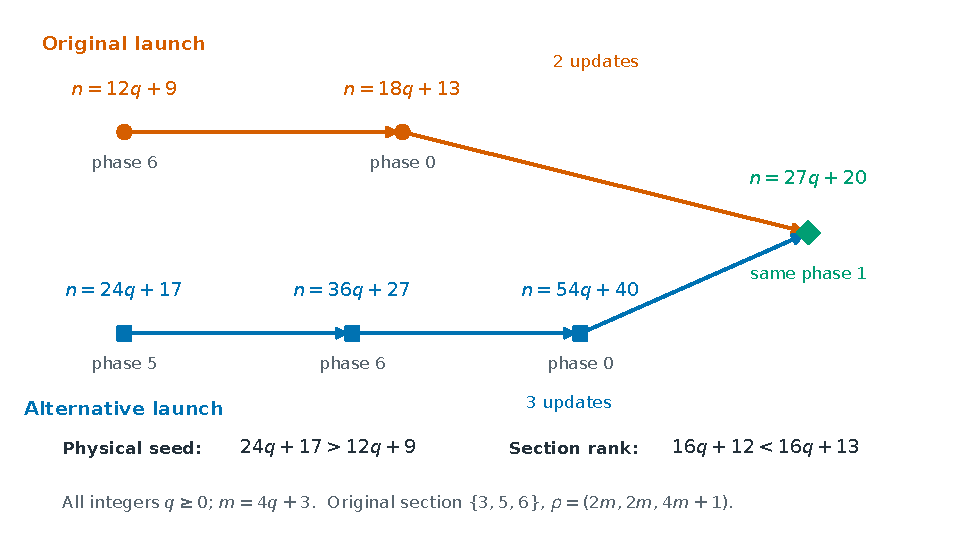
\includegraphics[width=0.93\linewidth]{figures/seven_step_merger.pdf}
\caption{The phase-correct merger used by the four-family reduction.
The two histories reach the same augmented state after different numbers
of updates. Their launch ranks differ by exactly one in $\rho$.
This figure concerns $\mathcal S$ and $\rho$; the alternative section
and rank in Section~\ref{sec:seven-three} are separate constructions.}
\label{fig:seven-merger}
\end{figure}

\paragraph{Reproduction.} Run
\begin{verbatim}
python3 certificates/seven_step/verify.py
python3 certificates/seven_step/test_mutations.py
\end{verbatim}
The first command reconstructs the physical certificates, compares
every field with the stored data, and checks an independent $T/U$
reconstruction on all fourteen phase--parity combinations. The second
tests rejection of defective and empty certificates. Both require
assertions enabled. The arbitrary-wait bound and least-rank induction
are written proofs.

\subsection{A second section with three residual families}
\label{sec:seven-three}

For the same forcing word and destination cycle take

\begin{equation}\label{eq:seven-new-section}
\begin{gathered}
 \mathcal S_* = \{(z,i):z=3m,\ m\ge1,\ i\in\{1,2,3,5\}\},
 \\
 W(m,i)=w_i m,\quad (w_1,w_2,w_3,w_5)=(4,7,4,5).
\end{gathered}
\end{equation}
The physical launch is still $s(m,i)=(3m-1+h_i,i)$, now with the
four indicated phases.  Write $P_*$ for the first strictly later visit
to $\mathcal S_*$.

\begin{theorem}[Three-family conditional capture]\label{thm:seven-three}
Every positive physical integer at every initial phase is captured by
\eqref{eq:seven-cycle} if and only if all three following statements hold:
\begin{align*}
 \mathrm{B1}:&\quad \operatorname{Cap}(s(2t,1)) &&(t\ge1),\\
 \mathrm{A3}:&\quad \operatorname{Cap}(s(4t+3,3)) &&(t\ge0),\\
 \mathrm{N03}:&\quad \operatorname{Cap}(s(8t+2,5)) &&(t\ge0).
\end{align*}
Every safe orbit enters $\mathcal S_*$ within eleven updates, and all
first returns from phases $1,2,3,5$ occur within $2,7,6,7$ updates,
respectively.  Outside the three families and five explicitly captured
states, $P_*$ strictly decreases the single natural-valued rank $W$.
The theorem does not prove any of the three universal capture hypotheses.
\end{theorem}

\paragraph{Uniform entry and bounded return.}
For entry, partition the phase-zero positive coordinate as
$z=1536q+r$, $0\le r<1536$, with $q\ge1$ for $r=0$ and $q\ge0$
otherwise.  The coefficient $1536=3\cdot2^9$ has more than enough
powers of two for five exact updates and retains a factor of three
throughout.  Consequently both parity and section membership are
constant on every propagated affine domain.  Independent physical
propagation gives the complete entry-time distribution
\[
 \begin{array}{c|rrrr}
 \text{first entry time}&1&2&3&5\\\hline
 \text{number of residue domains}&1024&384&64&64.
 \end{array}
\]
The counts sum to 1536.  Alignment from an arbitrary launch phase to
phase zero costs at most six updates, proving the stated bound of eleven.

For first returns, start with the entire domain $z=3m$ at each marked
phase.  Whenever the next parity is not fixed, split the free parameter
into its even and odd cases.  A growing branch $G$ and a shrinking branch
$S$ in the positive coordinate have the formulas
\[
 G_i(z)=\frac{3z+h_i}{2}\quad(z\equiv h_i\pmod2),\qquad
 S_i(z)=\frac{z+1-h_i}{2}\quad(z\not\equiv h_i\pmod2).
\]
These formulas describe branches of the prescribed $T/U$ schedule;
the branch is determined by the input parity. After $g$ growing updates,
the free coefficient is $3^{g+1}$: each parity split supplies the factor
of two consumed by that update. It is odd and divisible by three,
justifying the next split and the constant test for section membership.
Stop a domain at its
first later marked phase with $3\mid z$.  This procedure terminates
within the stated caps and produces the 43 domains in
Table~\ref{tab:seven-three-cylinders}.  At each source phase the
domains are pairwise disjoint and their dyadic widths sum to one.
Since all moduli are powers of two and bounded by the corresponding
$2^{L_i}$, this is an exhaustive finite partition of the positive
integers, not a density-only coverage claim.

As a separate reconstruction, partition $m$ modulo $2^{L_i}$ with
$(L_1,L_2,L_3,L_5)=(2,7,6,7)$, and propagate the original physical
recurrence, checking safety and the absence of an earlier section hit.
There are $4+128+64+128=324$ full-modulus input domains.  Each reproduces
the endpoint and time of its unique adaptive domain.  The two procedures
share the forcing and the section definition, but use different
coordinates and different partitions.

\begingroup
\small
\setlength{\tabcolsep}{7pt}
\begin{longtable}{rllllr}
\caption{The complete first-return partition for $\mathcal S_*$. All rows have
$t\ge0$, except $t\ge1$ when the displayed input is a multiple of $t$
with zero constant. The trace records every update, so its length is the
return time. The final column is $W_{\rm out}-W_{\rm in}$.}
\label{tab:seven-three-cylinders}\\
\toprule
$i$&input $m$&output $(m',j)$&trace&rank change&updates\\\midrule
\endfirsthead
\toprule
$i$&input $m$&output $(m',j)$&trace&rank change&updates\\\midrule
\endhead
\bottomrule
\endfoot
1&$2t$&$(3t,2)$&\texttt{G}&$13t$&1\\
1&$4t+1$&$(3t+1,3)$&\texttt{SG}&$-4t$&2\\
1&$4t+3$&$(t+1,3)$&\texttt{SS}&$-12t-8$&2\\
2&$2t$&$(3t,3)$&\texttt{G}&$-2t$&1\\
2&$8t+3$&$(9t+4,5)$&\texttt{SGG}&$-11t-1$&3\\
2&$8t+5$&$(3t+2,5)$&\texttt{SSG}&$-41t-25$&3\\
2&$8t+7$&$(3t+3,5)$&\texttt{SGS}&$-41t-34$&3\\
2&$64t+1$&$(9t+1,1)$&\texttt{SSSSGG}&$-412t-3$&6\\
2&$64t+17$&$(3t+1,1)$&\texttt{SSSSSG}&$-436t-115$&6\\
2&$64t+25$&$(9t+4,1)$&\texttt{SSSGGS}&$-412t-159$&6\\
2&$64t+33$&$(3t+2,1)$&\texttt{SSSSGS}&$-436t-223$&6\\
2&$64t+41$&$(9t+6,1)$&\texttt{SSSGSG}&$-412t-263$&6\\
2&$64t+49$&$(t+1,1)$&\texttt{SSSSSS}&$-444t-339$&6\\
2&$64t+57$&$(27t+25,1)$&\texttt{SSSGGG}&$-340t-299$&6\\
2&$128t+9$&$(9t+1,2)$&\texttt{SSSGSSG}&$-833t-56$&7\\
2&$128t+73$&$(3t+2,2)$&\texttt{SSSGSSS}&$-875t-497$&7\\
3&$4t$&$(3t,5)$&\texttt{SG}&$-t$&2\\
3&$4t+1$&$(3t+1,5)$&\texttt{GS}&$-t+1$&2\\
3&$4t+3$&$(9t+7,5)$&\texttt{GG}&$29t+23$&2\\
3&$32t+2$&$(9t+1,1)$&\texttt{SSGGS}&$-92t-4$&5\\
3&$32t+6$&$(3t+1,1)$&\texttt{SSSGS}&$-116t-20$&5\\
3&$32t+10$&$(9t+3,1)$&\texttt{SSGSG}&$-92t-28$&5\\
3&$32t+18$&$(27t+16,1)$&\texttt{SSGGG}&$-20t-8$&5\\
3&$32t+22$&$(9t+7,1)$&\texttt{SSSGG}&$-92t-60$&5\\
3&$32t+30$&$(3t+3,1)$&\texttt{SSSSG}&$-116t-108$&5\\
3&$64t+14$&$(3t+1,2)$&\texttt{SSSSSG}&$-235t-49$&6\\
3&$64t+26$&$(9t+4,2)$&\texttt{SSGSSG}&$-193t-76$&6\\
3&$64t+46$&$(t+1,2)$&\texttt{SSSSSS}&$-249t-177$&6\\
3&$64t+58$&$(3t+3,2)$&\texttt{SSGSSS}&$-235t-211$&6\\
5&$8t$&$(9t,1)$&\texttt{GSG}&$-4t$&3\\
5&$8t+2$&$(27t+7,1)$&\texttt{GGG}&$68t+18$&3\\
5&$8t+3$&$(9t+4,1)$&\texttt{SGG}&$-4t+1$&3\\
5&$8t+5$&$(3t+2,1)$&\texttt{SSG}&$-28t-17$&3\\
5&$8t+6$&$(9t+7,1)$&\texttt{GGS}&$-4t-2$&3\\
5&$8t+7$&$(3t+3,1)$&\texttt{SGS}&$-28t-23$&3\\
5&$16t+4$&$(3t+1,2)$&\texttt{GSSS}&$-59t-13$&4\\
5&$16t+9$&$(3t+2,2)$&\texttt{SSSG}&$-59t-31$&4\\
5&$16t+12$&$(9t+7,2)$&\texttt{GSSG}&$-17t-11$&4\\
5&$32t+17$&$(3t+2,3)$&\texttt{SSSSG}&$-148t-77$&5\\
5&$128t+1$&$(9t+1,5)$&\texttt{SSSSSGG}&$-595t$&7\\
5&$128t+33$&$(3t+1,5)$&\texttt{SSSSSSG}&$-625t-160$&7\\
5&$128t+65$&$(3t+2,5)$&\texttt{SSSSSGS}&$-625t-315$&7\\
5&$128t+97$&$(t+1,5)$&\texttt{SSSSSSS}&$-635t-480$&7\\
\end{longtable}
\endgroup


\paragraph{The finite exceptions and the induction.}
On a row $(Mt+r,i)\mapsto(At+b,j)$, the rank change is
\[
 W_{\rm out}-W_{\rm in}=(w_jA-w_iM)t+w_jb-w_ir.
\]
Exactly three rows have positive leading coefficient.  They are
\begin{center}
\begin{tabular}{llll}\toprule
Family&launch&first return&rank change\\\midrule
B1&$(2t,1)$&$(3t,2)$&$13t$\\
A3&$(4t+3,3)$&$(9t+7,5)$&$29t+23$\\
N03&$(8t+2,5)$&$(27t+7,1)$&$68t+18$\\\bottomrule
\end{tabular}
\end{center}
They grow on their whole legal domains.  Every other row has a negative
leading coefficient.  Solving its affine inequality on the entire legal
parameter ray leaves just
\[
 E=\{(1,1),(1,3),(1,5),(3,5),(5,3)\}
\]
as possible failures of strict descent.  Their capture times are
$4,2,0,14,16$ updates, respectively.  The first three have the physical
chains $(2,1)\to(1,2)\to(3,3)\to(4,4)\to(2,5)$ and its indicated
suffixes; $(2,5)$ is already on the destination cycle.  The longer two
chains, with phases advancing by one at each arrow, are
\begin{align*}
 (8,5):\quad&8,5,7,11,17,27,40,20,11,16,8,4,3,4,2,\\
 (15,3):\quad&15,22,11,18,8,4,2,2,0,0,1,1,2,1,3,4,2.
\end{align*}
Both end at phase five with physical value two.  The second chain
also illustrates why the convention at zero matters: it passes through
zero and continues, exactly as the forcing requires.

\begin{proof}[Proof of Theorem~\ref{thm:seven-three}]
The three families consist of positive physical states, so universal
capture implies their capture.  Conversely assume the three universal
statements.  If a safe orbit failed capture, uniform entry would give
a failed state in $\mathcal S_*$.  Choose such a state of least positive
integer rank $W$.  It is not in $E$, whose exact capture chains were
given above, and it is not in a residual family by hypothesis.
Its first return therefore strictly decreases $W$.  The return state
also fails capture, since its future is a suffix of the same orbit.
This contradicts minimality.  Every safe state is consequently captured.
\end{proof}

\paragraph{What changed relative to the four-family reduction.}
A3 is the old family S00.  At phase five, N03 is the subfamily
$m\equiv2\pmod8$ of the old even family S01.  The new section also
introduces B1 at phase one.  For the old S02 and S03 launches, it records
earlier endpoints
\[
 (32t+3,5)\xrightarrow{3}(36t+4,1),\qquad
 (128t+115,5)\xrightarrow{3}(144t+130,1).
\]
Their $W$-drops are $16t-1$ and $64t+55$.  The first is positive for
$t\ge1$; its remaining input $(3,5)$ belongs to $E$.  This explains
concretely how changing the section helps.  It does not prove capture
of those old families without the new hypotheses: a rank decrease
reduces an induction obligation but needs the common well-founded
argument to finish it.  Combining individual drops from $\rho$ and
$W$ without constructing one compatible order would not be valid.

\begin{proposition}[Three growing domains are optimal for this section]
\label{prop:seven-three-barrier}
Among positive phase-affine ranks
$R(m,i)=a_i m+b_i$ on $\mathcal S_*$, at least three of nine specified
disjoint first-return domains have a positive leading rank change.
The rank $W$ attains three growing domains in the complete 43-domain
partition.  The optimality assertion concerns this section and these
direct first-return comparisons.
\end{proposition}
\begin{proof}
Use the following three cycles of constraints, taking each labeled
edge from Table~\ref{tab:seven-three-cylinders}:
\[
 \begin{array}{c|c|c}
 \text{phase cycle}&\text{successive branch traces}&
       \text{product of slopes}\\\hline
 1\to2\to5\to1&G,\ SGG,\ GGS&243/128\\
 1\to3\to5\to1&SG,\ GS,\ GGG&243/128\\
 2\to3\to5\to2&G,\ GG,\ GSSG&243/128
 \end{array}
\]
Each edge is a different row of the disjoint partition.  If all three
leading rank changes in one cycle were nonpositive, multiplying
$a_jA\le a_iM$ around it would imply that the product of its slopes
$A/M$ is at most one.  Each displayed product is greater than one.
Thus each cycle contributes a different row with positive leading
coefficient; fixed offsets $b_i$ cannot cancel its growth for arbitrarily
large parameters.  The exact rank-change column proves attainment by
$W$.  These are cycles of inequalities on weights, not asserted
periodic trajectories satisfying every successive guard.
\end{proof}

\paragraph{Reproduction.}
\path{certificates/seven_step/three_family.py} regenerates
\path{three_family.json}, including the 43 affine rows, five finite
chains, independent physical reconstruction, entry times, and nine
obstruction witnesses. All 43 rows in \path{SevenRows.lean} agree with
the printed table after the parameter shift on zero-residue rows.

The Lean proof checks entry modulo 192 in at most six updates for
positive physical seeds at every phase. The eleven-update proof above
also covers safe zero states. Section~\ref{sec:formal-scope} gives the
formal three-family equivalence. The optimality proof above is written.

